

This section motivates the use of dynamic core fusion and its impact on performance and energy.
It also shows that loop optimizations have a significant performance impact when fusing cores.

\subsection{Dynamic Core Fusion}
\begin{figure}[t]
    \centering
    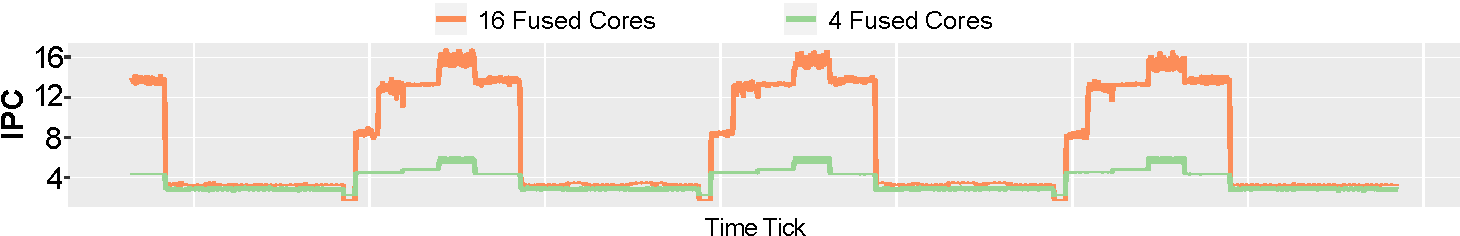
\includegraphics[width=\textwidth]{cases-paper/graphics/motivation/disp_opt_4_16_3.pdf}
    \caption{IPC of a typical benchmark (Disparity from SD-VBS) when executing on a fused 4 or 16 core processor.} 
    \label{fig:disp_ex}
\end{figure}
\begin{figure}[t]
    \centering
    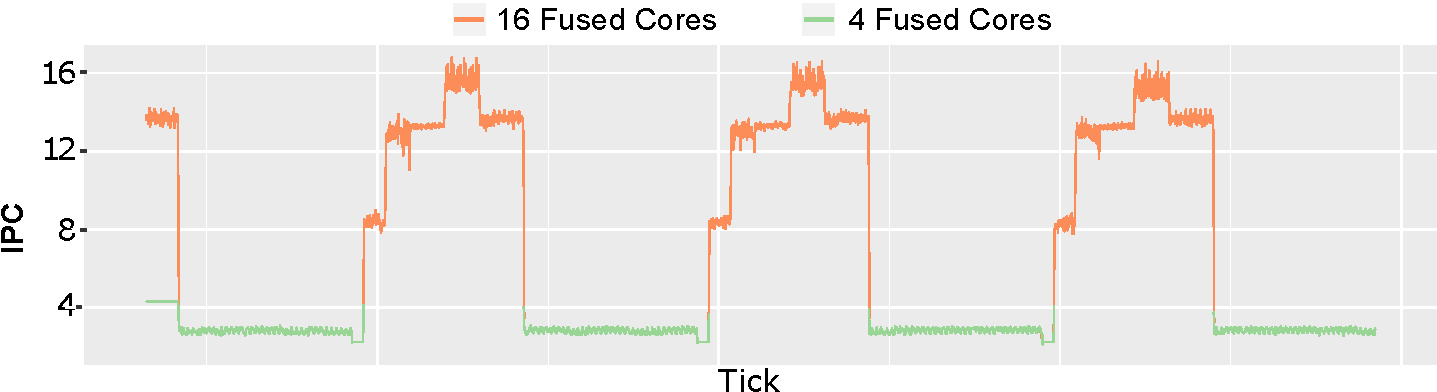
\includegraphics[width=\textwidth]{cases-paper/graphics/motivation/motiv3merge.pdf}
    \caption{Example of ideal switching between 4 and 16 cores on a DMP for the Disparity benchmark.} 
    \label{fig:ideal_switch}
\end{figure}
Previous work in core fusion has focused on delivering performance improvements~\cite{ipek2007CoreFusion,kim2007tflex} and demonstrated how to predict static core fusion~\cite{micolet2016dmpstream}.
A static fusion will fuse cores into a single logical core (LC) and execute a thread on this new core.
As evident from this prior work, fusion improves the performance of the program by maximizing speed.
However, as will be shown, static core fusion may not be the perfect match for all situations.

Figure~\ref{fig:disp_ex} plots the Instruction Per Cycle (IPC) performance variation over the execution of the \bm{Disparity} Benchmark from the San-Diego Vision Benchmark Suite (SD-VBS)~\cite{sdvbs} on a fused 4 core and 16 core processor.
On 4 cores, the performance oscillates between an IPC of 2 and 6 depending on the phase while on 16 cores the IPC can be as high as 16.
More importantly, for some phases (half of the time), the same level of IPC is achieved, around 3 IPC, whether the program runs on 4 or 16 cores.
A DMP could exploit this to minimize energy consumption while maximizing performance by fusing only 4 cores during the low IPC phases and fusing 16 cores during the high IPC phases as seen in Figure~\ref{fig:ideal_switch}.

\subsection{Code Optimizations}
When cores are fused they execute blocks of instructions in parallel on each physical core in the LC.
In order to obtain the best results, large blocks must be generated as this leads to a higher IPC on the LC~\cite{micolet2016dmpstream}.
The optimizations applied include aggressive loop unrolling, inlining and replacing conditional statements with either software predication or architecture-level predication.
These optimizations are well known and do not require any structural modifications of the program.

\begin{figure}[t]
    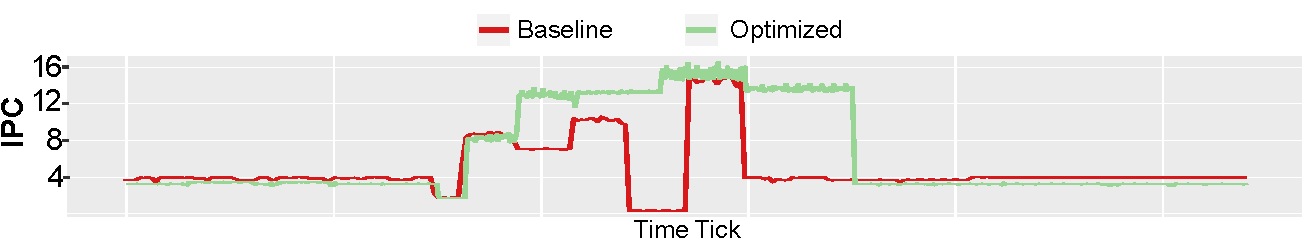
\includegraphics[width=\textwidth]{cases-paper/graphics/motivation/code_opt_3.pdf}
    \caption{Impact of loop transformations on fused cores for the Disparity benchmark.} 
    \label{fig:compmotiv}
\vspace{5mm}
\end{figure}
Figure~\ref{fig:compmotiv} illustrates the impact of applying loop transformations compared to a standard compiler not specifically tuned for an EDGE architecture.
As can be seen, the impact of these transformations can be large and are necessary to sustain a high IPC for a long enough period.
More details about the loop transformations are given in section~\ref{sec:opt} but this example illustrates the need for careful tuning of the compiler to achieve high performance on such an architecture.

\subsection{Summary}
This section has shown that programs exhibit phases with various amount of ILP available.
A dynamic multicore processor can take advantage of this property to fuse a large number of cores for the high-ILP phases and fuse a smaller number of cores when ILP drops to conserve energy.
The section also illustrated the importance of fine-tuned code transformations to achieve sustained performance and increase the potential for fusing cores.
The next section will study in more details the expected impact of fusion using an analytical model.

